% Copyright 2007 by Marco Barisione
% Copyright 2011 by Henricus Bouwmeester
%
% This file may be distributed and/or modified
%
% 1. under the LaTeX Project Public License and/or
% 2. under the GNU Public License.
%
% If you want to specifically use the Helvetica Neue font which is the 
% font defined in the Branding and Identity Standards for UC Denver,
% you will need to use xelatex to compile as well as commenting out 
% the current font commands in the preamble then uncomment the fontspec
% package as well as the fontspec command after \begin{document}

\documentclass[10pt]{beamer}
\usefonttheme{serif}
% \documentclass[10pt,hyperref={pdfpagelabels=false}]{beamer}
\usepackage{amsmath,amsfonts,mathrsfs}
\usepackage{colortbl}

\newcommand\blfootnote[1]{%
  \begingroup
  \renewcommand\thefootnote{}\footnote{#1}%
  \addtocounter{footnote}{-1}%
  \endgroup
}

\newcommand{\etal}{{\it et al.\ }}
\newcommand{\bs}[1]{\boldsymbol{#1}}

\makeatletter
\renewcommand{\@makefnmark}{\hbox{\textsuperscript{\tiny{\@thefnmark}}}}
\makeatother

% set font to Helvetica
%\usepackage[T1]{fontenc}
%\usepackage[scaled=0.92]{helvet}
%\renewcommand*\familydefault{\sfdefault} %% Only if the base font of the document is to be sans serif
% \usepackage{fontspec}

\newif\ifuseblack
% for black theme, this should be
%     \useblacktrue
% for the white theme, this should be
%     \useblackfalse
\useblacktrue

\usetheme[pageofpages=of,                    % String used between the current page and the
                                             % total page count.
          bullet=circle,                     % Use circles instead of squares for bullets.
          titleline=true,                    % Show a line below the frame title.
          showdate=true,                     % show the date on the title page
          alternativetitlepage=true,         % Use the fancy title page.
          %titlepagelogo=../images/culogo, % Logo for the first page.
          titlepagelogo=../images/CUAnschutz_c_clr, % Logo for the first page.
          % Logo for the header on first page.
          \ifuseblack
             headerlogo=../images/pubHealth_tt2_rgb_rv_tp,
          \else
             headerlogo=../images/csph_biostatistics,    % Logo for white background.
          \fi
          watermark=../images/watermark,               % Watermark used in every page.
          watermarkheight=50pt,              % Height of the watermark.
          watermarkheightmult=6,             % The watermark image is 6 times bigger
                                             % than watermarkheight.
          ]{UCDenver}

\ifuseblack
   \usecolortheme{ucdblack}
\else
   \usecolortheme{ucdwhite}
\fi

% ============================================================================ %
% Document info
% ============================================================================ %

\author{Peter E. DeWitt}
\title[Intro to Git]{Git: Distributed Version Control \\ {\small An
Introduction}}
\institute{
\includegraphics[height=1.5\fontcharht\font`\B]{../images/culogo} AMC $|$ CSPH $|$ Biostats}
\date{25 February 2015}

\logo{
\includegraphics[height=15pt]{../images/csph_biostatistics}}

% ============================================================================ %
% Document
% ============================================================================ %

\begin{document} 
  \watermarkoff

  \begin{frame}[t,plain]
    \titlepage
  \end{frame}

  \begin{frame}[t]
    \frametitle{Outline}
    \framesubtitle{Why? and little bit of How?}
    \tableofcontents[hideallsubsections] 
  \end{frame}

  \section{Welcome: Why Git?}
  \begin{frame}[t]{Acknowledgements and Other Resources}
    \begin{itemize}
      \item The first part of this presentation was inspired by, and copies
        from, `Git and
        Github\footnote{\url{github.com/rstudio/webinars/blob/master/2015-02/git-github.pdf}},' a webinar presented by Hadley Wickham.
      \item {\it Pro Git} 2nd
        edition\footnote{\url{http://git-scm.com/book/en/v2}}, best possible
        single source reference.
      \item This presentation highlights parts of the first three chapters from
        {\it Pro Git}.
      \item A branching model I subscribe to:
        \url{http://nvie.com/posts/a-successful-git-branching-model/}
    \end{itemize} 
  \end{frame}

  \begin{frame}[t]
    \frametitle{Git}
    \begin{itemize}
      \item Can be difficult and frustrating to learn
      \item Payoff: {\bf Safety} and {\bf Community}
      \item 
    \end{itemize}
    ``Failures, repeated failures, are finger posts on the road to achievement.
    One fails forward towards success.'' -- C.S.\ Lewis
  \end{frame}

  \begin{frame}[t]{A Story in Pictures}
    \framesubtitle{http://www.phdcomics.com/comics/archive.php?comicid=1323} 
    \begin{center}
      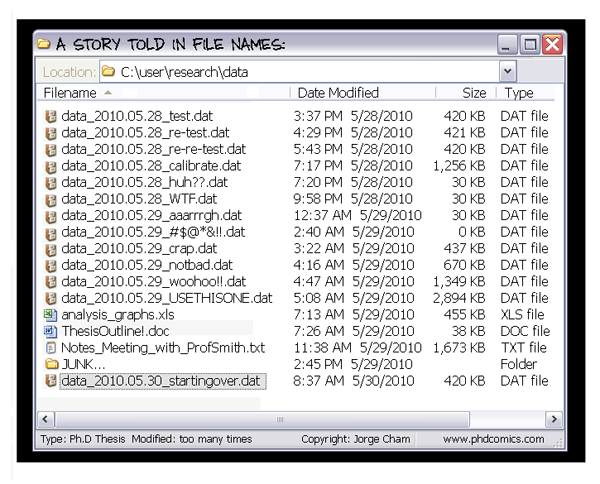
\includegraphics[height=2.75in]{../images/phd052810s.png} 
    \end{center}
  \end{frame}

  \begin{frame}[t]{A Story in Pictures}
    \framesubtitle{http://www.phdcomics.com/comics/archive.php?comicid=1531} 
    \begin{center}
      
\includegraphics[height=2.75in]{../images/phd101212s.png} 
    \end{center}
  \end{frame}

  \begin{frame}[t]
    \frametitle{Changes}
    The history of a project can be viewed as a series of changes:
    \begin{center}
      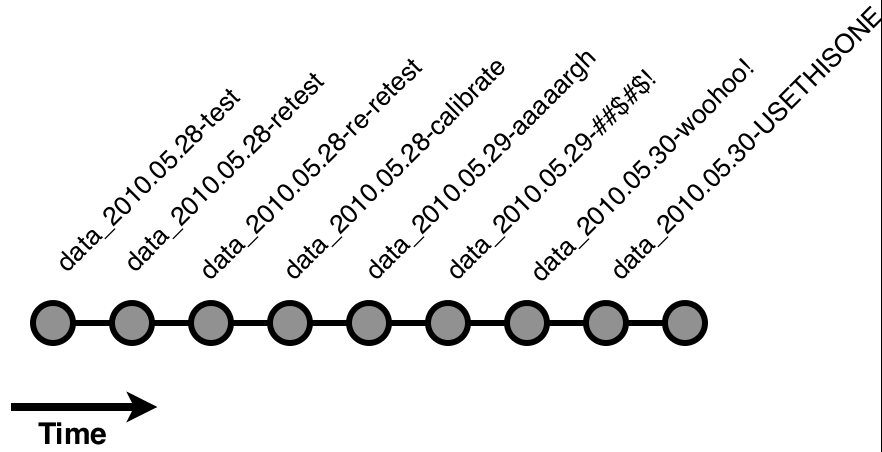
\includegraphics[height=2.00in]{../images/from-wickham-01.png} 
    \end{center} 
  \end{frame}

  \begin{frame}[t]
    \frametitle{Changes}
    \begin{itemize}
      \item A unique identifier
      \item What changed?
      \item When did it change?
      \item Who changed it?
      \item Why did it change?
      \item[]
      \item Difficult to coordinate with multiple files
    \end{itemize}
  \end{frame}

  \begin{frame}[t]
    \frametitle{Changes}
    With git, each change ({\bf commit}) is given a unique identifier, a {\bf
    sha}.
    \begin{center}
      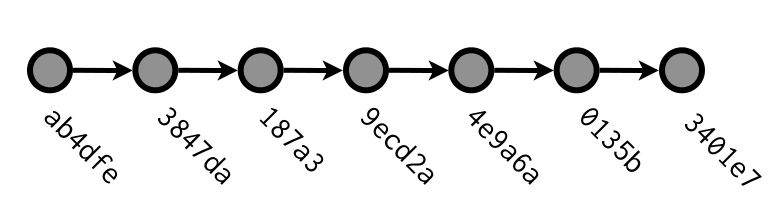
\includegraphics[width=0.98\textwidth]{../images/from-wickham-02.png} 
    \end{center} 

    \begin{itemize} 
      \item sha is a 40 digit long hexadecimal value $> 1.46 \times 10^{48}$
        unique values
      \item sha is a key into a database that provides the author, date, and a
        description
    \end{itemize} 
  \end{frame}

  \begin{frame}[t]
    \frametitle{Changes}
    You can also name individual commits.
    \begin{center}
      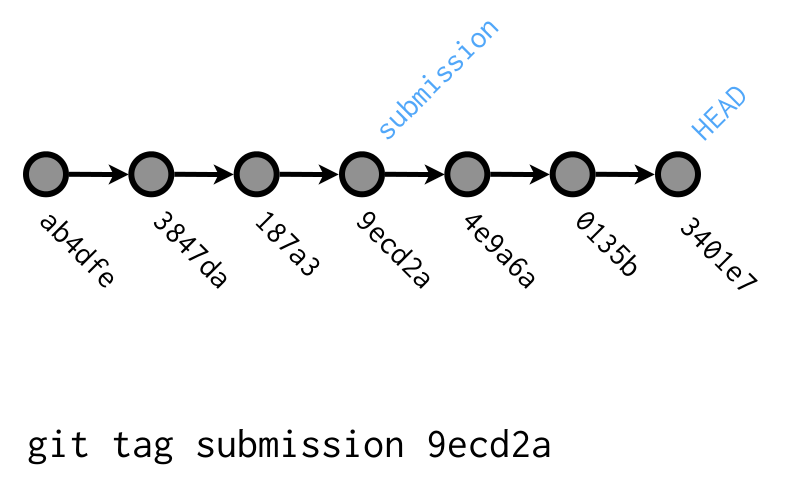
\includegraphics[height=2.00in]{../images/from-wickham-03.png} 
    \end{center} 

    \begin{itemize} 
      \item {\tt HEAD} is the location the working directory is set to.
      \item {\tt submission} is an example of a {\bf tag}
    \end{itemize} 
  \end{frame}

  \begin{frame}[t]
    \frametitle{Changes}
    Then see exactly what was changed 
    \begin{center}
      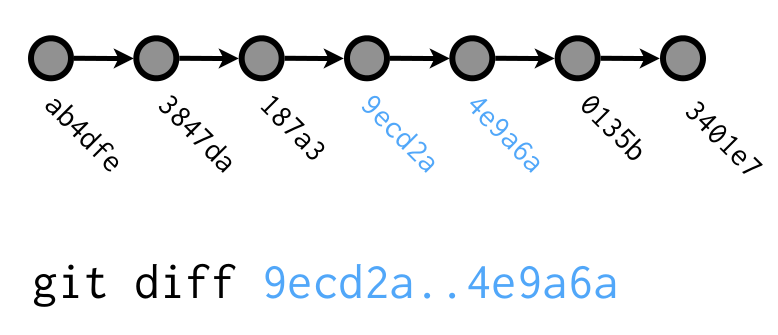
\includegraphics[height=2.00in]{../images/from-wickham-04.png} 
    \end{center} 
  \end{frame}

  \begin{frame}[t]
    \frametitle{Changes}
    You can revert to a previous change with git checkout
    \begin{center}
      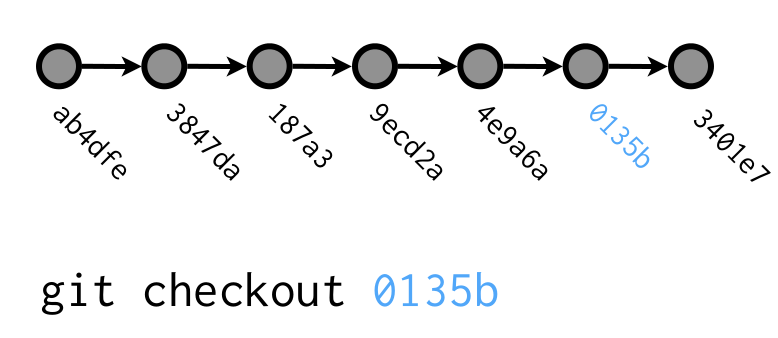
\includegraphics[height=2.00in]{../images/from-wickham-05.png} 
    \end{center} 
  \end{frame}

  \begin{frame}[t]
    \frametitle{Changes}
    That allows you to undo mistakes
    \begin{center}
      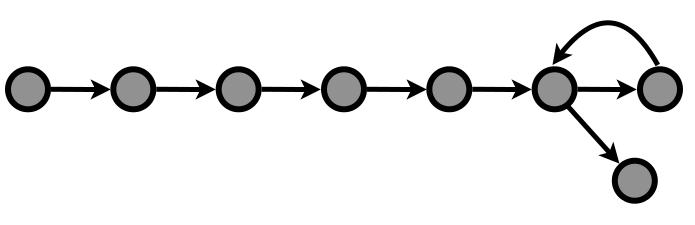
\includegraphics[width=0.98\textwidth]{../images/from-wickham-06.png} 
    \end{center} 
  \end{frame}



  \section{Closing}
  \begin{frame}[t]{Outline}
    \tableofcontents[currentsection,hideallsubsections]
  \end{frame}

  \begin{frame}[t] 
    \frametitle{Closing}
    \begin{center}
    Thank you for your time.

    \vspace{1in}

    The floor is open for questions and comments.
    \end{center} 
  \end{frame}

\end{document}

